% Created 2020-07-03 vie 15:41
% Intended LaTeX compiler: pdflatex
\documentclass[presentation,aspectratio=169]{beamer}
\usepackage[utf8]{inputenc}
\usepackage[T1]{fontenc}
\usepackage{graphicx}
\usepackage{grffile}
\usepackage{longtable}
\usepackage{wrapfig}
\usepackage{rotating}
\usepackage[normalem]{ulem}
\usepackage{amsmath}
\usepackage{textcomp}
\usepackage{amssymb}
\usepackage{capt-of}
\usepackage{hyperref}
\usepackage{khpreamble}
\usepackage{amssymb}
\usepackage{tcolorbox}
\DeclareMathOperator{\shift}{q}
\DeclareMathOperator{\diff}{p}
\usetheme{default}
\author{Kjartan Halvorsen}
\date{2020-07-03}
\title{Control Computarizado - Discretización del proceso continuo}
\hypersetup{
 pdfauthor={Kjartan Halvorsen},
 pdftitle={Control Computarizado - Discretización del proceso continuo},
 pdfkeywords={},
 pdfsubject={},
 pdfcreator={Emacs 26.3 (Org mode 9.3.6)}, 
 pdflang={English}}
\begin{document}

\maketitle

\section{Intro}
\label{sec:org73ca54b}
\begin{frame}[label={sec:orgd4e92a6}]{El mundo según el controlador discreto}
\begin{center}
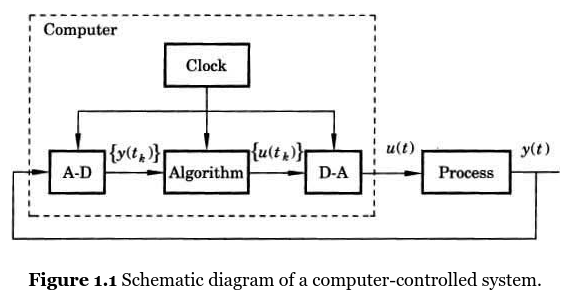
\includegraphics[width=0.7\linewidth]{../../figures/fig1-1-schematic.png}
\end{center}
{\footnotesize Åström \& Wittenmark \textit{Computer-controlled systems}}
\end{frame}
\begin{frame}[label={sec:orge64a893}]{Discretización del proceso}
\begin{center}
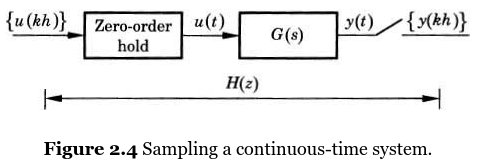
\includegraphics[width=0.6\linewidth]{../../figures/fig2-4.png}
\end{center}
{\footnotesize Åström \& Wittenmark \textit{Computer-controlled systems}}
\end{frame}
\section{Zero-order hold, or step-invariant sampling preview}
\label{sec:org598e7fb}
\begin{frame}[label={sec:org6eedb7e}]{Discretización invariante al escalón (\emph{step-invariant} o \emph{zero-order-hold sampling})}
El idea es muestrear la respuesta del escalón del sistema continuo para obtener un modelo discreto que es \alert{exacto} (en los instantes de muestreo) para señales de entrada que son combinaciones de escalones (funciones constantes por partes)

\begin{center}
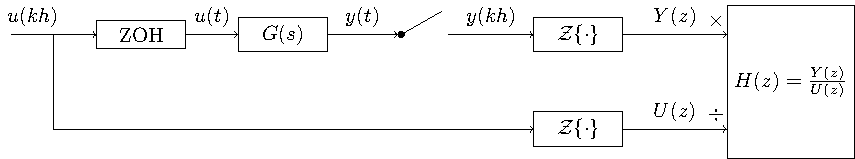
\includegraphics[width=0.99\linewidth]{../../figures/invariant-sampling.pdf}
\end{center}

\[ u(kh) = \begin{cases} 1, & k \ge 0\\0, & k<0 \end{cases} \]
\end{frame}

\begin{frame}[label={sec:org5527da7}]{Porqué discretización invariante al escalón?}
Una función constante por partes, como produce el retenedor de orden cero, puede ser escrito como una suma de escalones retrasados:

\begin{center}
  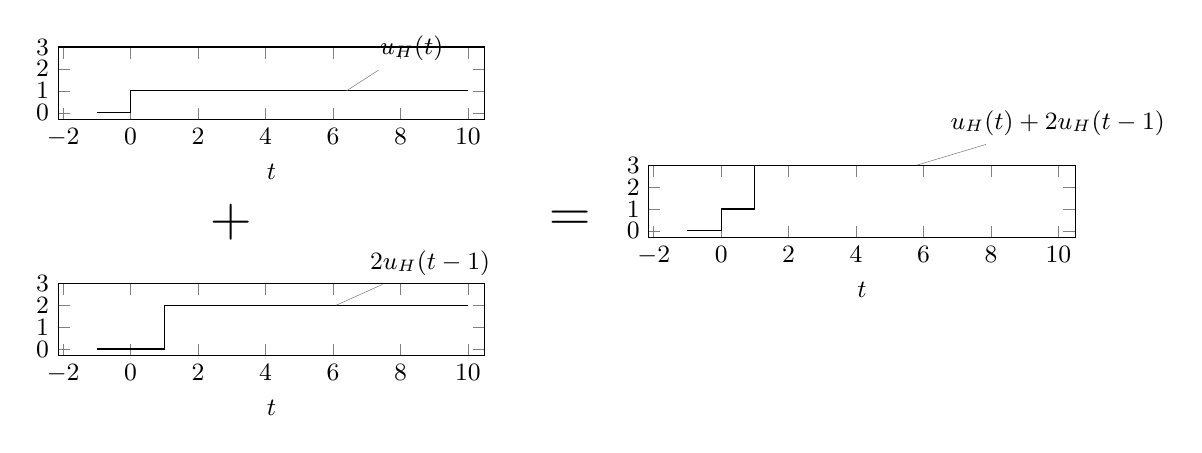
\begin{tikzpicture}
    \small
    \begin{axis}[
      clip = false,
      width=7cm,
      height=2.5cm,
      yshift=1.5cm,
      xlabel={$t$},
      ylabel={},
      xmax=10.5,
      ymax=3,
      ]
      \addplot+[black, no marks] coordinates {(-1,0) (0,0) (0,1) (10,1) } node[pos=0.7,coordinate, pin=40:$u_H(t)$] {};
    \end{axis}
    \begin{axis}[
      clip=false,
      width=7cm,
      height=2.5cm,
      yshift=-1.5cm,
      xlabel={$t$},
      ylabel={},
      xmax=10.5,
      ymax=3,
      ]
      \addplot+[black, no marks] coordinates {(-1,0) (1,0) (1,2) (10,2) } node[pos=0.7,coordinate, pin=40:$2u_H(t-1)$] {};;
    \end{axis}
    \begin{axis}[
      clip=false,
      width=7cm,
      height=2.5cm,
      xshift=7.5cm,
      xlabel={$t$},
      ylabel={},
      xmax=10.5,
      ymax=3,
      ]
      \addplot+[black, no marks] coordinates {(-1,0) (0,0) (0,1) (1,1) (1,3) (10,3) }  node[pos=0.7,coordinate, pin=40:$u_H(t) + 2u_H(t-1)$] {};;
    \end{axis}

    \node at (2.2,0.2) {\huge  +};
    \node at (6.5,0.2) {\huge  =};

  \end{tikzpicture}
\end{center}
\end{frame}

\begin{frame}[label={sec:orgfcd7088}]{Porqué discretización invariante al escalón?}
Trabajamos con sistemas discretos LTI, entonces la respuesta de una suma de escalones retardados es la misma suma de respuestas de escalón retardados.

\begin{center}
  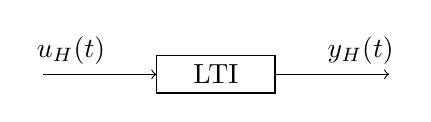
\begin{tikzpicture}[node distance=20mm, block/.style={rectangle, draw, minimum width=15mm, }]

    \node[coordinate] (input) {};
    \node[block, right of=input, node distance=22mm] (lti) {LTI};
    \node[coordinate, right of=lti, node distance=22mm] (output) {};

    \draw[->] (input) -- node[above, near start] {$u_H(t)$} (lti);
    \draw[->] (lti) -- node[above, near end] {$y_H(t)$} (output);
  \end{tikzpicture}
\end{center}
Si la respuesta de un escalón unitario del sistema es \(y_H(t)\), la señal de entrada  
\(u(t) = \sum_{i} \alpha_i u_H(t-\tau_i)\) va a dar la respuesta \[y(t)=?\]
\end{frame}

\begin{frame}[label={sec:org0f6aeb3}]{Porqué discretización invariante al escalón?}
Trabajamos con sistemas discretos LTI, entonces la respuesta de una suma de escalones retardados es la misma suma de respuestas de escalón retardados.

\begin{center}
  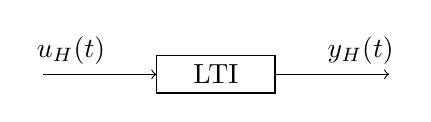
\begin{tikzpicture}[node distance=20mm, block/.style={rectangle, draw, minimum width=15mm, }]

    \node[coordinate] (input) {};
    \node[block, right of=input, node distance=22mm] (lti) {LTI};
    \node[coordinate, right of=lti, node distance=22mm] (output) {};

    \draw[->] (input) -- node[above, near start] {$u_H(t)$} (lti);
    \draw[->] (lti) -- node[above, near end] {$y_H(t)$} (output);
  \end{tikzpicture}
\end{center}
Si la respuesta de un escalón unitario del sistema es \(y_H(t)\), la señal de entrada  
\(u(t) = \sum_{i} \alpha_i u_H(t-\tau_i)\) va a dar la respuesta \[y(t)=\sum_{i} \alpha_i u_H(t-\tau_i)\]


\begin{tcolorbox}
   Si el método de discretización es exacto para una señal de entrada en forma de un escalón, va a ser exacto para señales que son constantes por partes. Este son el tipo de señales que produce el retenedor de orden cero. 
\end{tcolorbox}
\end{frame}



\section{Procedimiento}
\label{sec:org551cdb7}
\begin{frame}[label={sec:org40383e7}]{Procedimiento de discretización invariante al escalón}
\begin{center}
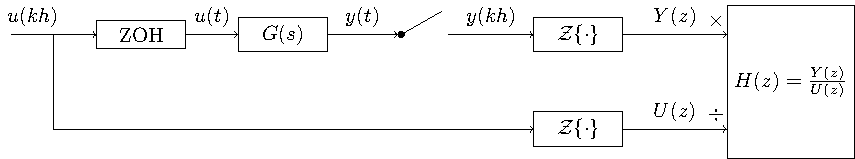
\includegraphics[width=0.99\linewidth]{../../figures/invariant-sampling.pdf}
\end{center}
\[ u(kh) = \begin{cases} 1, & k \ge 0\\0, & k<0 \end{cases} \]

\begin{tcolorbox}
\[ H(z) = \frac{z-1}{z} \ztrf{\mathcal{L}^{-1}\{ \frac{G(s)}{s} \}} \]
\end{tcolorbox}
\end{frame}

\begin{frame}[label={sec:org0ec1399}]{Ejemplo: Motor DC con retraso}
\begin{center}
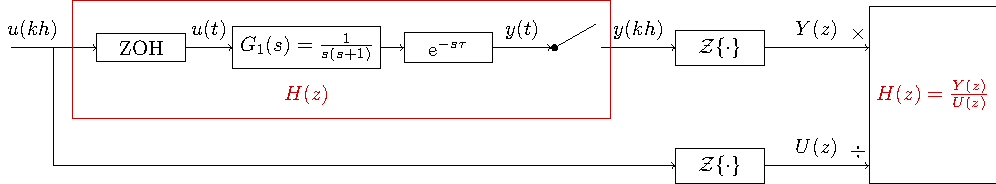
\includegraphics[width=0.89\linewidth]{../../figures/invariant-sampling-dcmotor.pdf}
\end{center}
\[ G(s) = G_1(s)\mathrm{e}^{-s\tau}\]

\begin{enumerate}
\item \alert{Respuesta sin retraso} \[ \frac{G(s)}{s} = \frac{1}{s^2(s+1)} = -\frac{1}{s} + \frac{1}{s^2} + \frac{1}{s+1} \]
\[ y_1(t) = \mathcal{L}^{-1} \{-\frac{1}{s} + \frac{1}{s^2} + \frac{1}{s+1}\} = u_H(t)\big(t-1+\mathrm{e}^{-t}\big).\]
\item \alert{Respuesta con retraso} \(y(t) = y_1(t-\tau) =  -u_H(t-\tau) + u_H(t-\tau)(t-\tau) + u_H(t-\tau)\mathrm{e}^{-(t-\tau)}\big)\)
\end{enumerate}
\end{frame}

\begin{frame}[label={sec:org6a28296}]{Ejemplo: Motor DC con retraso}
Asumiendo \(\tau = nh\)
\[ \ztrf{f(kh-nh)} = z^{-n}\ztrf{f(kh)}.\]
\begin{enumerate}
\setcounter{enumi}{2}
\item \alert{Transformada z de la respuesta sin retraso, muestreada} 
Usando las transformadas
\begin{align*}
u_H(kh) \quad &\overset{\mathcal{Z}}{\longleftrightarrow} \quad \frac{z}{z-1}\\
u_H(kh)kh \quad &\overset{\mathcal{Z}}{\longleftrightarrow} \quad \frac{zh}{(z-1)^2}\\
u_H(kh)\mathrm{e}^{-a(kh)} \quad &\overset{\mathcal{Z}}{\longleftrightarrow} \quad \frac{z}{z-\mathrm{e}^{-ah}}
\end{align*}
\[Y_1(z) = -\frac{z}{z-1} + \frac{zh}{(z-1)^2} + \frac{z}{z-\mathrm{e}^{-h}}\]
\end{enumerate}
\end{frame}

\begin{frame}[label={sec:org1961aec}]{Ejemplo: Motor DC con retraso}
\begin{enumerate}
\setcounter{enumi}{3}
\item \alert{Transformada z de la respuesta retresada}
\[ Y(z) = z^{-n} \left(-\frac{z}{z-1} + \frac{zh}{(z-1)^2} + \frac{z}{z-\mathrm{e}^{-h}}\right)\]
\item \alert{Diviendo por la transformada z del escalón} 
\begin{align*}
H(z) &= \frac{Y(z)}{U(z)} = \frac{z-1}{z} z^{-n} \left(-\frac{z}{z-1} + \frac{zh}{(z-1)^2} + \frac{z}{z-\mathrm{e}^{-h}}\right)\\
&= z^{-n} \left( -1 + \frac{h}{z-1} + \frac{z-1}{z-\mathrm{e}^{-h}} \right)\\
&= \frac{ z\big( h-1+\mathrm{e}^{-h}\big) - \big(\mathrm{e}^{-h}(1+h) - 1\big)}{z^n(z-1)(z-\mathrm{e}^{-h})}
\end{align*}
\end{enumerate}
\end{frame}

\begin{frame}[label={sec:org54625db}]{Ejemplo: Motor DC con retraso}
\[ G(s) = \frac{\mathrm{e}^{-s(nh)}}{s(s+1)} \quad \longrightarrow \quad
   H(z) = \frac{ z\big( h-1+\mathrm{e}^{-h}\big) - \big(\mathrm{e}^{-h}(1+h) - 1\big)}{z^n(z-1)(z-\mathrm{e}^{-h})}\]
\alert{Actividad} Determina el cero y los polos si \(n=1\) y \(h=0.2\). Marcalos (cero con  \tikz \draw (1ex,.7ex) circle (.8ex); y polos con \(\times\)) en los diagramas correspondientes.
\begin{columns}
\begin{column}{0.4\columnwidth}
\begin{tikzpicture}
\node[red] at (-1.5,2) {\Large $s$-plane};
\draw[->] (-2,0) -- (1,0); 
\draw[->] (0,-2) -- (0,2);
\end{tikzpicture}
\end{column}


\begin{column}{0.6\columnwidth}
\begin{tikzpicture}
\node {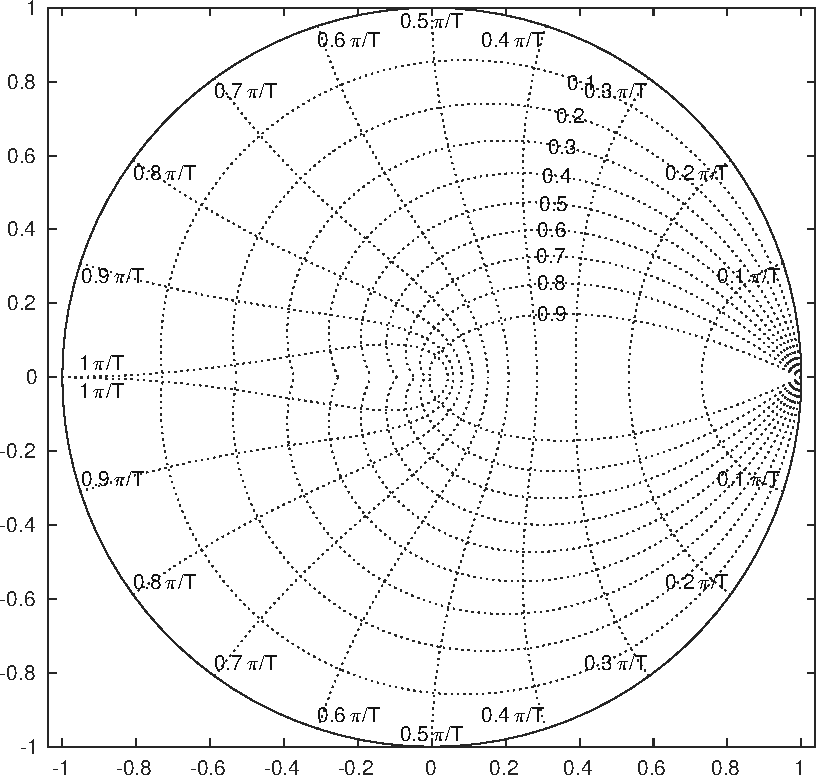
\includegraphics[height=0.6\textheight]{../../figures/zgrid-crop}};
\node[red] at (2.5,2.2) {\Large $z$-plane};
\end{tikzpicture}
\end{column}
\end{columns}
\end{frame}

\begin{frame}[label={sec:orga0f2b6d}]{Ejercico: Sistema de primer orden}
\alert{Actividad} Discretiza el sistema 
\[ G(s) = \frac{1}{s + a} \]
usando el método de discretización invariante al escalón.
\begin{center}
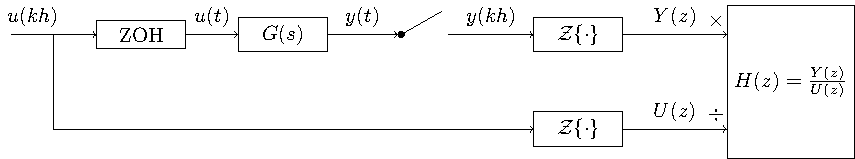
\includegraphics[width=0.69\linewidth]{../../figures/invariant-sampling.pdf}
\end{center}

\begin{tcolorbox}
\[ H(z) = \frac{z-1}{z} \ztrf{\mathcal{L}^{-1}\{ \frac{G(s)}{s} \}} \]
\end{tcolorbox}
\end{frame}

\begin{frame}[label={sec:orgf2c9e99}]{Ejercico: Sistema de primer orden - solución}
\begin{enumerate}
\item Respuesta al escalón
\[y(t) = \mathcal{L}^{-1}\{G(s)/s\} = \mathcal{L}^{-1}\left\{\frac{1}{a}\big(\frac{1}{s} - \frac{1}{s+a}\big)\right\} = \frac{1}{a}(1 - \mathrm{e}^{-at}).\]
\item Transformada z de la respuesta muestreada
\[ Y(z) = \ztrf{y(kh)} = \frac{1}{a} \ztrf{1 - \mathrm{e}^{-akh}} = \frac{1}{a} \left( \frac{z}{z-1} - \frac{z}{z-\mathrm{e}^{-ah}} \right)\]
\item División con \(H(z)\)
\begin{align*}
 H(z) &=  \frac{1}{a} \frac{z-1}{z} \left( \frac{z}{z-1} - \frac{z}{z-\mathrm{e}^{-ah}} \right)
     = \frac{1}{a} \left( 1 - \frac{z-1}{z-\mathrm{e}^{-ah}}\right)\\
     &= \frac{\frac{1}{a}\big((z-\mathrm{e}^{-ah}) - (z-1)\big)}{z-\mathrm{e}^{-ah}}
      = \frac{\frac{1}{a}(1-\mathrm{e}^{-ah})}{z-\mathrm{e}^{-ah}}
\end{align*}
\end{enumerate}
\end{frame}

\section{Mapeo del plano s al plano z}
\label{sec:orgc493860}
\begin{frame}[label={sec:org3f29dd1}]{La transformada de Laplace de una señal muestreada}
Nota:
\begin{align*}
F_s(s) &=  \sum_{k=0}^{\infty} f(kh) \left(\mathrm{e}^{-sh}\right)^k\quad \text{transformada de Laplace}\\
F(z) &= \sum_{k=0}^{\infty} f(kh) z^{-k} \quad \text{transformada z}
\end{align*}

\begin{tcolorbox}
La transformada z de una señal muestreada corresponde a su transformada de Laplace bajo la relación 
\[ z = \mathrm{e}^{sh}\]
entre el dominio $s$ de la transformada de Laplace y el dominio $z$ de la tranformada z.
\end{tcolorbox}
\end{frame}



\begin{frame}[label={sec:orgcadcc63}]{Mapeo del plano \(s\) al plano \(z\)}
\begin{tcolorbox}
\[ z = \mathrm{e}^{sh} \qquad \Leftrightarrow \qquad  s = \frac{1}{h} \ln z\]
\end{tcolorbox}

\alert{Ejemplo importante} Semiplano izquierdo del plano \(s\) : \(s = a + i\omega, \; a < 0\)
\[ z = \mathrm{e}^{sh} = \mathrm{e}^{(a + i\omega)h} = \mathrm{e}^{ah} \mathrm{e}^{i\omega h}, \quad |z| = |\mathrm{e}^{ah}|\, |\mathrm{e}^{i\omega h}| = |\mathrm{e}^{ah}| < 1, \; a < 0\]
\end{frame}

\begin{frame}[label={sec:org771a244}]{Ejercicio}
\alert{Actividad en pareja} Encuentra las correspondencias usando \(z = \mathrm{e}^{sh}\)

   \begin{center}
   \begin{tikzpicture}[node distance=40mm]
   \node (spl) {Plano $s$};
   \node[right of=spl] (sp1) {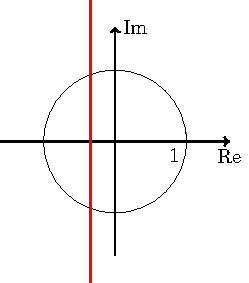
\includegraphics[height=0.3\textheight]{../../figures/imaginary-plane-vertical-line}};
   \node[right of=sp1] (sp2) {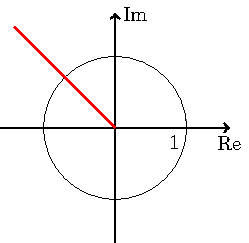
\includegraphics[height=0.3\textheight]{../../figures/imaginary-plane-diagonal-line}};
   \node[right of=sp2] (sp3) { 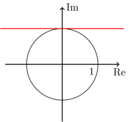
\includegraphics[height=0.3\textheight]{../../figures/imaginary-plane-horizontal-line}};
   \node[below of=spl, node distance=30mm] (zpl) {Plano \(z\)};
   \node[right of=zpl] (zp1) {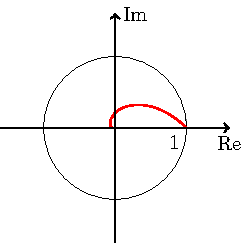
\includegraphics[height=0.3\textheight]{../../figures/imaginary-plane-diagonal-line-map}};
   \node[right of=zp1] (zp2) {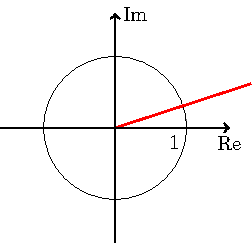
\includegraphics[height=0.3\textheight]{../../figures/imaginary-plane-horizontal-line-map}};
   \node[right of=zp2] (zp3) {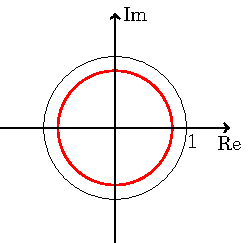
\includegraphics[height=0.3\textheight]{../../figures/imaginary-plane-circle-z}};

   %\draw[<->, thick, orange] (sp1) to (zp3);
   %\draw[<->, thick, blue] (sp2) to (zp1);
   %\draw[<->, thick, green!80!black] (sp3) to (zp2);
 \end{tikzpicture}
\end{center}
\end{frame}

\begin{frame}[label={sec:org0a3b880}]{Ejercicio - solución}
   \begin{center}
   \begin{tikzpicture}[node distance=40mm]
   \node (spl) {Plano $s$};
   \node[right of=spl] (sp1) {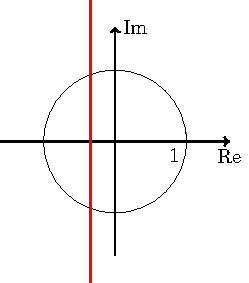
\includegraphics[height=0.3\textheight]{../../figures/imaginary-plane-vertical-line}};
   \node[right of=sp1] (sp2) {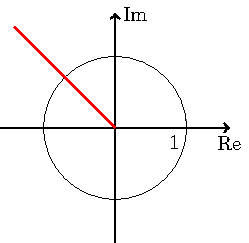
\includegraphics[height=0.3\textheight]{../../figures/imaginary-plane-diagonal-line}};
   \node[right of=sp2] (sp3) { 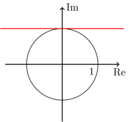
\includegraphics[height=0.3\textheight]{../../figures/imaginary-plane-horizontal-line}};
   \node[below of=spl, node distance=30mm] (zpl) {Plano \(z\)};
   \node[right of=zpl] (zp1) {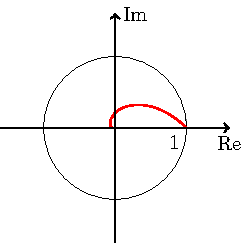
\includegraphics[height=0.3\textheight]{../../figures/imaginary-plane-diagonal-line-map}};
   \node[right of=zp1] (zp2) {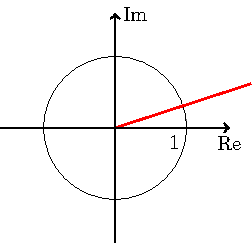
\includegraphics[height=0.3\textheight]{../../figures/imaginary-plane-horizontal-line-map}};
   \node[right of=zp2] (zp3) {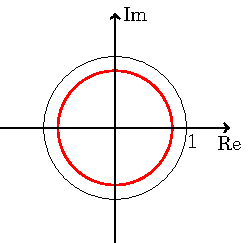
\includegraphics[height=0.3\textheight]{../../figures/imaginary-plane-circle-z}};

   \draw[<->, thick, orange] (sp1) to (zp3);
   \draw[<->, thick, blue] (sp2) to (zp1);
   \draw[<->, thick, green!80!black] (sp3) to (zp2);
 \end{tikzpicture}
\end{center}
\end{frame}
\end{document}